\documentclass[a4paper, 14pt]{extarticle}

\usepackage{../generalPreamble}
\usepackage{../reportFormat}

% chktex-file 44

\begin{document}

\begin{titlepage}
    \centering
    {\bfseries
        \uppercase{
            Минобрнауки России \\
            Санкт-Петербургский государственный \\
            Электротехнический университет \\
            \enquote{ЛЭТИ} им. В.И.Ульянова (Ленина)\\
        }
        Кафедра ИБ

        \vspace{\fill}
        \uppercase{Лабораторная работа №1} \\
        по дисциплине \enquote{Криптография и защита информации} \\
        Тема: Изучение классических шифров средствами RailFence, Scytale, Caesar
    }

    \vspace{\fill}
    \begin{tabularx}{0.8\textwidth}{l X c r}
        Студент гр. 6304 & & \underline{\hspace{3cm}} & Корытов П.В.\\
        Преподаватель & & \underline{\hspace{3cm}} & Племянников А.К.
    \end{tabularx}

    \vspace{1cm}
    Санкт-Петербург \\
    \the\year{}
\end{titlepage}

\newpage

\section*{Цель работы}
Исследовать шифры Rail Fence, Scytale, Caesar и получить практические навыки работы с ними, в том числе и в программном продукте Cryptool 1 и 2.

\section{Шифр Rail Fence}
\subsection{Описание шифра}
Тип шифра --- перестановка.

В шифре Изгороди открытый текст разбивается на определенное количество строк. В каждой строке поочередно записывается одна буква подобно изгороди, зашифрованный текст составляется при чтении строки за строкой. Например, при разбиении открытого текста ``0123456789'' на 3 строки шифрование выглядит следующим образом:

\begin{tabularx}{0.8\textwidth}{XXXXXXXXXXXX}
\multicolumn{10}{c}{Разбиение на строки} &  & Шифротекст \\
0 &  &  &  & 4 &  &  &  & 8 &  &  &  \\
 & 1 &  & 3 &  & 5 &  & 7 &  & 9 & =\textgreater{} & 0481357926 \\
 &  & 2 &  &  &  & 6 &  &  &  &  & 
\end{tabularx}

Для увеличения криптостойкости используют смещение. Пример для смещения 2:

\begin{tabularx}{0.8\textwidth}{XXXXXXXXXXXXX}
\multicolumn{10}{c}{Разбиение на строки} &  &  & Шифротекст \\
--- &  &  &  & 3 &  &  &  & 7 &  &  &  &  \\
 & --- &  & 2 &  & 4 &  & 6 &  & 8 &  & =\textgreater{} & 2613579048 \\
 &  & 1 &  &  &  & 5 &  &  &  & 9 &  & 
\end{tabularx}

Таким образом, ключ шифра --- число строк ($N_r$) и смещение ($O$). Так как $ O \le N_r < l$, где $l$ --- длина сообщения, сложность атаки грубой силы:
\begin{equation}
    N_{bf} < l^2
\end{equation}

\subsection{Задание}
\begin{enumerate}
    \item Найти шифр в CrypTool 1: Encrypt/Decrypt-> Symmetric (Classis).
    \item Создать файл с открытым текстом, содержащим последовательность цифр.
    \item Запустить шифр и выполнить зашифровку и расшифровку созданного текста несколько раз.
    \item Установить, как влияют на шифрование параметры Number of Rows и Offset.
    \item Зашифровать и расшифровать текст, содержащий только фамилию (транслитерация латиницей) вручную и с помощью шифра при Number of Rows>2, Offset≥2. Убедиться в совпадении результатов.
    \item Создайте шифровку для варианта Offset=0 и Number of Rows≤ и передайте коллеге слева для расшифровки.
    \item Определите ключ методом ``грубой сил'' и расшифруйте полученный от коллеги шифротекст.
\end{enumerate}
\subsection{Выполнение задания}
\begin{enumerate}
    \item В CrypTool найден шифр Rail Fence. 
    \begin{figure}[h]
        \centering
        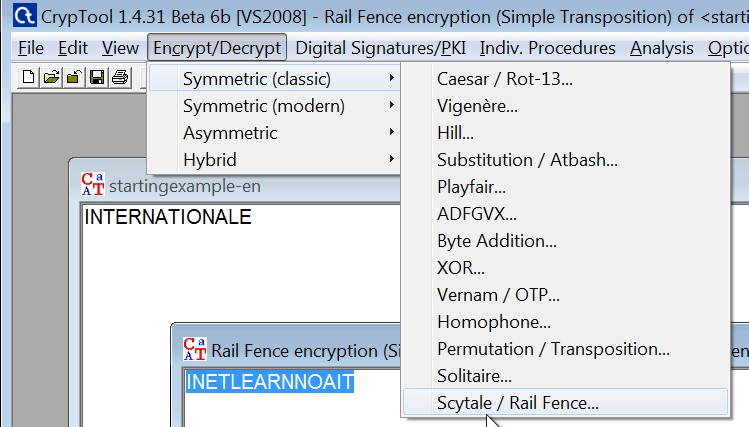
\includegraphics[width=0.7\textwidth]{./img/S002.jpg}
        \caption{Шифр Rail Fence в CrypTool}%
        \label{img:fence:1}
    \end{figure}
    \begin{figure}[h]
        \centering
        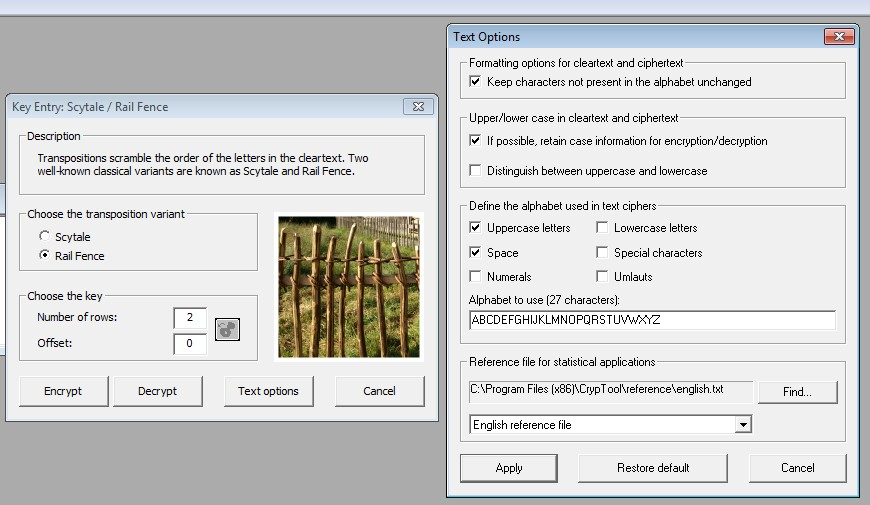
\includegraphics[width=0.9\textwidth]{./img/S005.jpg}
        \caption{Опции шифровния в CrypTool 1}%
        \label{img:fence:2}
    \end{figure}

    \item Создан файл с открытым текстом, содержащим последовательность цифр 12345678900987654321
    \item Произведена зашифровка и расшифровка созданного текста. Результаты на рисунке~\ref{img:fence:3}
    \begin{figure}[h]
        \centering
        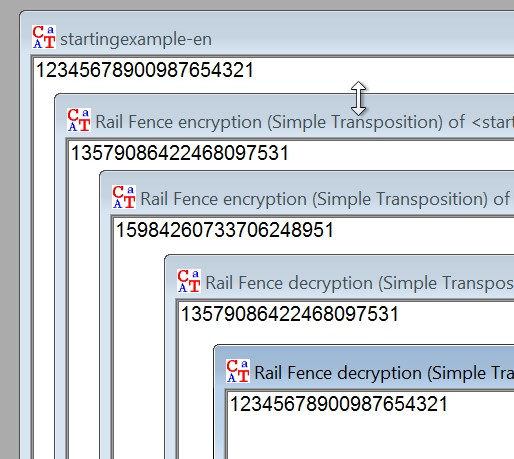
\includegraphics[width=0.5\textwidth]{./img/S003.jpg}
        \caption{Зашифровка и расшифровка}%
        \label{img:fence:3}
    \end{figure}
    \item Number of rows в шифре --- число строк, Offset --- смещение. Так, зашифровка $123456$ с параметрами $(2,0)$ превращает его в $135246$ --- сначала записываются четные цифры, затем --- нечетные. Если поставить $(2,1)$, то результат --- $246135$, т.к. в таком случае первая цифра --- нечетная.
    \item Зашифрована и расшифрована вручную фамилия автора --- \texttt{KORYTOV} --- с параметрами $(3,2)$\\
    \begin{tabularx}{0.8\textwidth}{XXXXXXXXXXX}
    --- &   &  &  & R &  &  &  & V &  &  \\
      & --- &  & O &  & Y &  & O &  & =\textgreater{} & RVOYOKT \\
      &   & K &  &  &  & T &  &  &  & 
    \end{tabularx}

    Смещение --- 2, длина текста --- 7 $\Rightarrow$ длина таблицы --- 9:\\
    \begin{tabularx}{0.8\textwidth}{XXXXXXXXX}
    --- &  &  &  & X &  &  &  & X \\
     & --- &  & X &  & X &  & X &  \\
     &  & X &  &  &  & X &  & 
    \end{tabularx}

    Подстановка шифротекста в вышеуказанную таблицу дает ответ:\\
    \begin{tabularx}{0.8\textwidth}{XXXXXXXXX}
    --- &  &  &  & R &  &  &  & V \\
     & --- &  & O &  & Y &  & O &  \\
     &  & K &  &  &  & T &  &  \\
    \multicolumn{9}{c}{$ \Downarrow $} \\
     &  & K & O & R & Y & T & O & V
    \end{tabularx}

    Как видно на рисунке~\ref{img:fence:3}, Зашифровка в CrypTool с такими же параметрами дает такие же результаты.
    \begin{figure}[h]
        \centering
        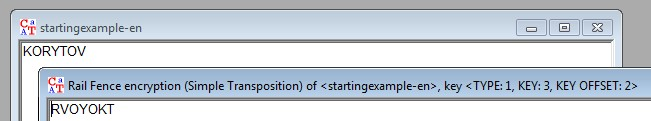
\includegraphics[width=0.8\textwidth]{./img/S006.jpg}
        \caption{Проверка зашифровки}%
        \label{img:fence:3}
    \end{figure}
    \item  Коллеге слева сгенерирована последовательность INTERNATIONALE и зашифрована с числом строк $8$: INETLEARNNOAIT.\@

Коллега расшифровывала последовательность меньше нескольких минут путём перебора числа строк.
    \item Полученная от коллеги слева последовательность: BKLIOINVNA.\@ Ход расшифровки представлен на рис.~\ref{img:fence:4}
    \begin{figure}[h]
        \centering
        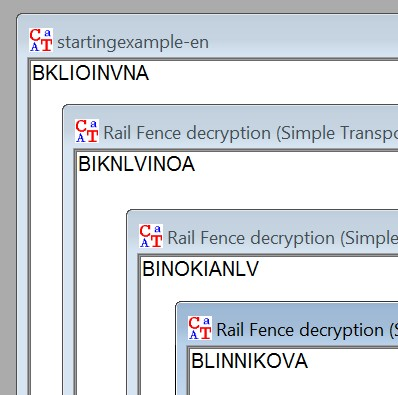
\includegraphics[width=0.5\textwidth]{./img/S001.jpg}
        \caption{Ход расшифровки последовательности}%
        \label{img:fence:4}
    \end{figure}
С 4-й попытки выяснено, что последовательность зашифрована с числом строк $4$. Соответственно, это ключ. 
\end{enumerate}


\section{Шифр ``Сцитала'' (Scytale)}
\subsection{Описание шифра}
Тип шифра --- перестановка.

В криптографии сцитала, известный также как шифр Древней Спарты, представляет собой прибор, используемый для осуществления перестановочного шифрования. Прибор состоит из цилиндра и узкой полоски пергамента, обматывавшейся вокруг него по спирали, на которой писалось сообщение. Иллюстрация, демонстрирующая работу данного шифра представлена на рисунке~\ref{img:theory:1}.

\begin{figure}[h]
    \centering
    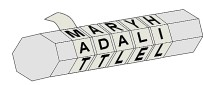
\includegraphics[width=0.4\textwidth]{img/S004.jpg}
    \caption{Иллюстрация шифра Сцитала}%
    \label{img:theory:1}
\end{figure}

Для расшифровки использовался цилиндр такого же диаметра, на который наматывался пергамент, чтобы прочитать сообщение.

Сложность атаки грубой силы в таком случае такая же, как и у шифра Rail Fence. Если убрать смещение (вряд ли оно применялось в Древней Греции) и учесть физические ограничения, число перебираемых вариантов едва ли превосходит несколько десятков.

\subsection{Задание}
\begin{enumerate}
    \item Найти шифр в CrypTool 1: Encrypt/Decrypt-> Symmetric (Classic).
    \item Создать файл с открытым текстом, содержащим последовательность цифр.
    \item Запустить шифр и выполнить зашифровку и расшифровку созданного текста несколько раз. 
    \item Установить, как влияют на шифрование параметры Number of Edges и Offset.
    \item Зашифровать и расшифровать текст содержащий только фамилию (транслитерация латиницей) вручную и с помощью шифра при Number of Edges > 2, Offset ≥ 2. Убедиться в совпадении результатов. 
    \item Взять в CrypTool 2 шаблон атаки на шифр методом ``грубой силы'' и модифицировать этот шаблон, заменив блок с шифротекстом на блок ввода открытого текста и блок зашифрования. Изучить принципы этой автоматической атаки.
\end{enumerate}
\subsection{Выполнение задания}
\begin{enumerate}
    \item В CrypTool 1 найден исследуемый шифр. Он находится в том же пункте, какой выбран на рисунке~\ref{img:fence:1}. Спецификация параметров такая же, как и на рисунке~\ref{img:fence:2}.
    \item Создан файл с открытым текстом: 0987654321123456789
    \item Произведена его зашифровка и расшифровка несколько раз. Результаты на рис.~\ref{img:scytale:1}
    \begin{figure}[h]
        \centering
        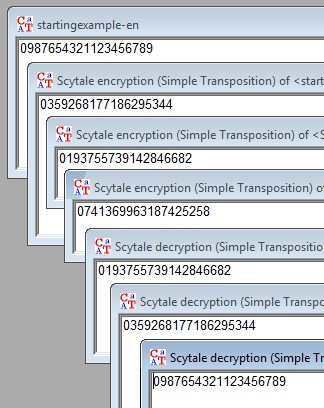
\includegraphics[width=0.5\textwidth]{img/S007.jpg}
        \caption{Зашифровка и расшифровка шифром Сцитала}%
        \label{img:scytale:1}
    \end{figure}
    \item Number of Rows в CrypTool --- количество граней цилиндра, Offset --- смещение от начальной грани.
    \item Фамилия автора --- KORYTOV --- зашифрована с параметрами $(3, 2)$.\\
    \begin{tabular}{ccc}
    --- & --- & K \\
    O & R & Y \\
    T & O & V \\
    \multicolumn{3}{c}{$\Downarrow$} \\
    \multicolumn{3}{c}{OTROKYV}
    \end{tabular}

    Расшифровка не составляет труда:\\
    \begin{tabularx}{0.8\textwidth}{XXXXX}
    --- & --- & K &  &  \\
    O & R & Y & =\textgreater{} & KORYTOV \\
    T & O & V &  & 
    \end{tabularx}

    CrypTool дает те же результаты.

    \item Проведена указанная модификация шаблона в CrypTool 2. В качестве текста взят первый куплет ``Интернационала'' в адаптации Билли Брэгга. 

    Принцип работы автоматической атаки заключается в переборе количества строк в указанном диапазоне (смещение не поддерживается) и в поиске известных слов в расшифровке. 

    Скриншот workspace CrypTool 2 в приложении А.
    
\end{enumerate}
\section{Шифр Цезаря (Caesar)}
\subsection{Описание шифра}
Шифр Цезаря — один из древнейших шифров. Шифр назван в честь римского императора Гая Юлия Цезаря, использовавшего его для секретной переписки.

Тип шифра --- замена.

\begin{itemize}
    \item Заменим буквы алфавита числами соответствующими их порядковым номерам в алфавите $0, 1, \ldots, n-1$.
    \item Представим символы открытого текста $P_i$ и шифротекста $C_i$
    \item Выбираем в качестве ключа числа $k$
    \item Шифрование: $C_i = (P_i + k) \bmod n$ 
    \item Расшифровка: $ P_i = (C_i - k) \bmod n $\\
\end{itemize}

Сложность атаки грубой силы --- $N_{bf} < n$

\subsection{Задание}
\begin{enumerate}
    \item Найти шифр в CrypTool 1: Encrypt/Decrypt-> Symmetric (Classic).
    \item Зашифровать и расшифровать текст, содержащий только фамилию (транслитерация латиницей) вручную и с помощью шифра с ключом, отличным от 0. Убедиться в совпадении результатов.
    \item Построить гистограмму частот букв английского языка по эталонному файлу English.txt (папка CrypTool/reference), используя утилиту из Analysis -> Tools for Analysis.
    \item Зашифровать ключом отличным от 0 файл CrypTool-en.txt (папка CrypTool / Examples).
    \item  Построить гистограмму частот букв в зашифрованном тексте, сравнить визуально гистограммы и подтвердить ключ зашифрования.
    \item Проверить гипотезу о значении ключа утилитой Analysis -> Symmetric Encryption (Classic)->Cipher Text Only->Caesar.
    \item Передать шифровку соседу слева для проведения подобной атаки.
\end{enumerate}

\subsection{Выполнение задания}
\begin{enumerate}
    \item Шифр найден в CrypTool 1. Параметры шифра указаны на рисунке~\ref{img:caesar:0}
    \begin{figure}[h]
        \centering
        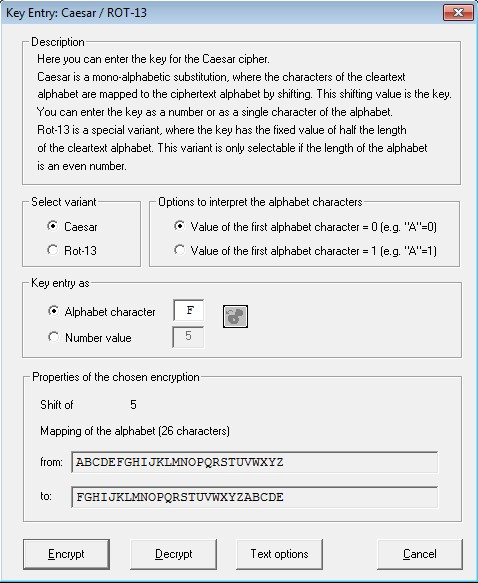
\includegraphics[width=0.8\textwidth]{img/S011.jpg}
        \caption{Спецификация параметров для шифра Цезаря}%
        \label{img:caesar:0}
    \end{figure}
    \item Фамилия автора ``KORYTOV'' зашифрована вручную с ключом $5$:\\
    \begin{tabular}{lllllllllllll}
    A & B & C & D & E & F & G & H & I & J & K & L & M \\
    V & W & X & Y & Z & A & B & C & D & E & F & G & H \\ \hline
    N & O & P & Q & R & S & T & U & V & W & X & Y & Z \\
    I & J & K & L & M & N & O & P & Q & R & S & T & U
    \end{tabular}

    Результат шифрования: ``FJMTOJQ''. Расшифровка дает исходный результат
    
    \item Построена гистограмма для указанного файла --- ``Повестки дня на XXI век'', ``Agenda 21''. Результат на рисунке~\ref{img:caesar:1}
    \begin{figure}[h]
        \centering
        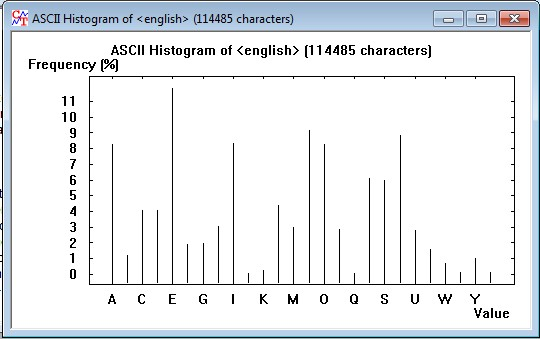
\includegraphics[width=0.8\textwidth]{img/S008.jpg}
        \caption{Распределение символов для Agenda 21}%
        \label{img:caesar:1}
    \end{figure}
    \item Предлагаемый файл зашифрован шифром Цезаря с ключом F.
    \begin{figure}[h]
        \centering
        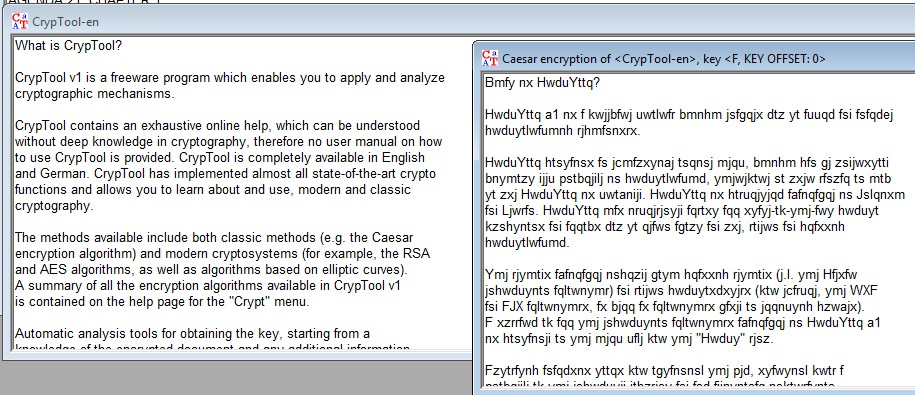
\includegraphics[width=\textwidth]{img/S009.jpg}
        \caption{Шифр Цезаря}%
        \label{img:caesar:2}
    \end{figure}
    \item Проверено визуальное совпадение диаграмм.
    \begin{figure}[h]
        \centering
        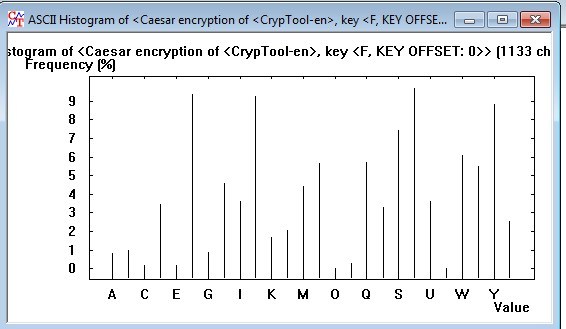
\includegraphics[width=0.8\textwidth]{img/S010.jpg}
        \caption{Диаграмма для зашифрованного текста}%
        \label{img:caesar:3}
    \end{figure}
    Диаграммы на рисунках~\ref{img:caesar:1} и~\ref{img:caesar:3} действительно похожи, однако из-за меньшего размера второго файла имеются расхождения.
    \item CrypTool 1, как и ожидалось, успешно подобрал ключ --- F.
\end{enumerate}

\FloatBarrier{}
\section*{Выводы}
\begin{itemize}
    \item Рассмотренные шифры --- симметричные, т.е. для шифрования и расшифрования используeтся один и тот же ключ
    \item Шифры Rail Fence и Scytale --- шифры перестановки, шифр Цезаря --- шифр замены
    \item Преимущество этих шифров --- возможность легкого использования без какого-либо вычислительного оборудования. Это сделало возможным их применение в Древнем Мире.
    \item Атака ``грубой силы'' на рассмотренные шифры не составляет труда и не намного сложнее, чем зашифровка сообщения.
    \item Наличие вычислительного оборудования делает взлом рассмотренных шифров тривиальной задачей.
    \item Частотный анализ позволяет провести эффективную атаку на шифр Цезаря; для Rail Fence и Scytale этот метод неприменим\\
\end{itemize}

Использованное ПО --- CrypTool 1 / CrypTool 2 в VirtualBox, neovim и \XeLaTeX{} для написания отчета.

\newpage

\begin{center}
    \bfseries
    \MakeUppercase{Приложение А}\\
    Среда CrypTool 2
\end{center}
\begin{figure}[h]
    \centering
    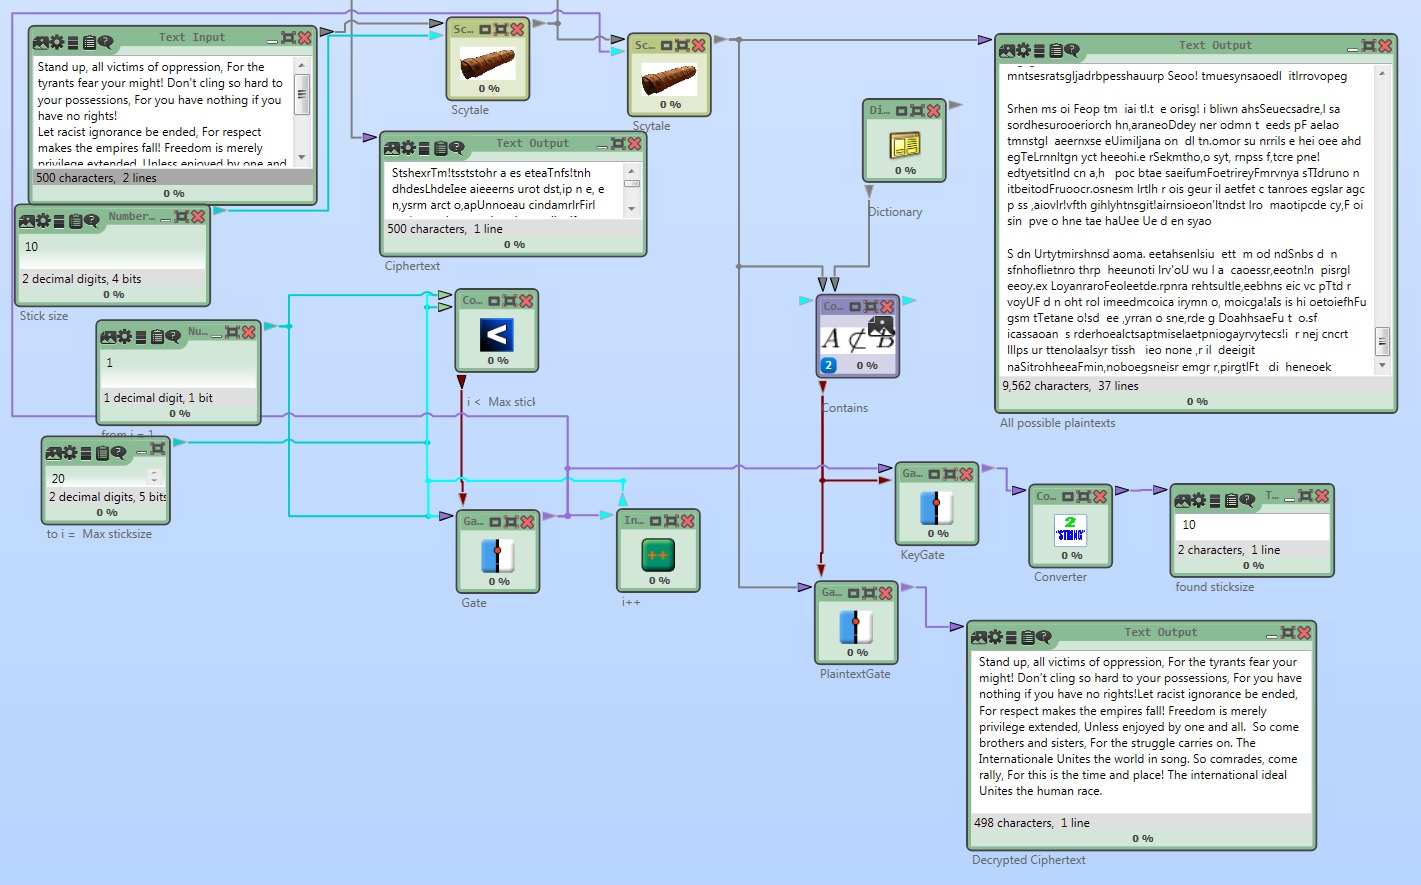
\includegraphics[angle=90,height=0.77\textheight]{img/L1.jpg}
\end{figure}

\end{document}
